%% 
%% Copyright 2007, 2008, 2009 Elsevier Ltd
%% 
%% This file is part of the 'Elsarticle Bundle'.
%% ---------------------------------------------
%% 
%% It may be distributed under the conditions of the LaTeX Project Public
%% License, either version 1.2 of this license or (at your option) any
%% later version.  The latest version of this license is in
%%    http://www.latex-project.org/lppl.txt
%% and version 1.2 or later is part of all distributions of LaTeX
%% version 1999/12/01 or later.
%% 
%% The list of all files belonging to the 'Elsarticle Bundle' is
%% given in the file `manifest.txt'.
%% 

%% Template article for Elsevier's document class `elsarticle'
%% with numbered style bibliographic references
%% SP 2008/03/01

%\documentclass[preprint,12pt]{elsarticle}
\documentclass[final,3p,times,review]{elsarticle}

%% Use the option review to obtain double line spacing
%% \documentclass[authoryear,preprint,review,12pt]{elsarticle}

%% Use the option review to obtain double line spacing
%% \documentclass[authoryear,preprint,review,12pt]{elsarticle}


% Add Reference title
\def\bibsection{\section*{References}}
% NOMENCLATURE
%\usepackage{framed} % Framing content
%\usepackage{multicol} % Multiple columns environment
%
%\usepackage{nomencl} % Nomenclature package
%\makenomenclature
%\setlength{\nomitemsep}{-\parskip} % Baseline skip between items
%
%\renewcommand*\nompreamble{\begin{multicols}{2}}
%\renewcommand*\nompostamble{\end{multicols}}

%% Use the options 1p,twocolumn; 3p; 3p,twocolumn; 5p; or 5p,twocolumn
%% for a journal layout:
%% \documentclass[final,1p,times]{elsarticle}
%% \documentclass[final,1p,times,twocolumn]{elsarticle}
%% \documentclass[final,3p,times]{elsarticle}
%% \documentclass[final,3p,times,twocolumn]{elsarticle}
%% \documentclass[final,5p,times]{elsarticle}
%% \documentclass[final,5p,times,twocolumn]{elsarticle}

%% For including figures, graphicx.sty has been loaded in
%% elsarticle.cls. If you prefer to use the old commands
%% please give \usepackage{epsfig}

%% The amssymb package provides various useful mathematical symbols
\usepackage{amssymb}
%% The amsthm package provides extended theorem environments
%% \usepackage{amsthm}

%%%%%%%%%%%% PACKAGE TO MAKE DOTTED LINES %%%%%%%%%%%%%%%%%%%%%%%%%%%%%%%%%%
\usepackage{array,arydshln}
%\setlength\dashlinedash{0.2pt}
%\setlength\dashlinegap{4.5pt}
%\setlength\arrayrulewidth{0.2pt}
%%%% Another combination of values
\setlength\dashlinedash{0.2pt}
\setlength\dashlinegap{1.5pt}
\setlength\arrayrulewidth{0.3pt}

%%%%%%%%%%%%%%% PACKAGE TO INCREASE THICKNESS OF TABLE ROW %%%%%%%%%%%%%%%%%%%%
\usepackage{array}

\newcolumntype{M}[1]{>{\centering\arraybackslash}m{#1}}
\newcolumntype{N}{@{}m{0pt}@{}}

%%%%%%%%%%% FOR BETTER REFERENCES %%%%%%%%%%%%%%%%%%%%%%%%
\usepackage[nodots]{numcompress}
\biboptions{square,sort&compress}
%%%%%%%%%%% TABLE DIMENSION %%%%%%%%%%%%%%%%%%%%%%%%
\usepackage{tabularx}

%%%%%%%%%%% LANDSCAPE %%%%%%%%%%%%%%%%%%%%%%%%
\usepackage{lscape}

\usepackage{amsmath}
\usepackage{amssymb}
%%%%%%%%%%%%%%%%%%%%%%%%%%%%%%%%%%%%%%%%%%%%%%%%%%%%%%%%%%%%%%%%%%%%%%%%%%%%

%% The lineno packages adds line numbers. Start line numbering with
%% \begin{linenumbers}, end it with \end{linenumbers}. Or switch it on
%% for the whole article with \linenumbers.
\usepackage{lineno}

\usepackage{graphicx,psfrag,subcaption,booktabs}

\usepackage{caption}

%%%%%%%%%%% PACKAGE FOR CHECK MARKS %%%%%%%%%%%%%%%%%%%%%%%%
\usepackage{tikz}
\def\checkmark{\tikz\fill[scale=0.4](0,.35) -- (.25,0) -- (1,.7) -- (.25,.15) -- cycle;} 

\journal{SolarEnergy}

\begin{document}
\linenumbers
\modulolinenumbers[1]
\begin{frontmatter}

%% Title, authors and addresses

%% use the tnoteref command within \title for footnotes;
%% use the tnotetext command for theassociated footnote;
%% use the fnref command within \author or \address for footnotes;
%% use the fntext command for theassociated footnote;
%% use the corref command within \author for corresponding author footnotes;
%% use the cortext command for theassociated footnote;
%% use the ead command for the email address,
%% and the form \ead[url] for the home page:
%% \title{Title\tnoteref{label1}}
%% \tnotetext[label1]{}
%% \author{Name\corref{cor1}\fnref{label2}}
%% \ead{email address}
%% \ead[url]{home page}
%% \fntext[label2]{}
%% \cortext[cor1]{}
%% \address{Address\fnref{label3}}
%% \fntext[label3]{}

\title{Steady-state and dynamic validation of a parabolic through collector model using the ThermoCycle Modelica library}

%% use optional labels to link authors explicitly to addresses:
%% \author[label1,label2]{}
%% \address[label1]{}
%% \address[label2]{}

%\author{Adriano Desideri, Martin van den broek, Gusev Sergei, Vincent Lemort, Sylvain Quoilin}
% Define authors %
%\fnref{fn1}}
\author[rvt]{Adriano Desideri\corref{cor1}}
\ead{adesideri@ulg.ac.be}
\cortext[cor1]{Corresponding author}
\author[rvt]{R\'emi Dickes}
\author[focal]{Javier Bonilla}
\author[focal]{Loreto Valenzuela}
\author[rvt]{Vincent Lemort}
\author[rvt]{Sylvain Quoilin}

\address[rvt]{Thermodynamics Laboratory, Aerospace and Mechanical Engineering Department, University of Li\`ege, B-4000, Li\`ege, Belgium}
\address[focal]{PSA-CIEMAT, Plataforma Solar de Almer\' ia - Centro de Investigaciones Energ\' eticas, MedioAmbientales y Tecnológicas, Crta. de Sen\' es s/n, 04200, Tabernas (Almer\' ia), Spain}
%
%
%
%
%
%
%
%
%
\address{}
%
\begin{abstract}
%% Text of abstract

\end{abstract}
%
\begin{keyword}
%% keywords here, in the form: keyword \sep keyword
Dynamic modelling, dynamic validation
%% PACS codes here, in the form: \PACS code \sep code

%% MSC codes here, in the form: \MSC code \sep code
%% or \MSC[2008] code \sep code (2000 is the default)

\end{keyword}

\end{frontmatter}

%% \linenumbers

%% main text
\section{Introduction}
\label{Intro}

%%%%%%%%%%%%%%%%%%%%%%%%%%%%%%%% NOMENCLATURE %%%%%%%%%%%%%%%%%%%%%%%%%%%%%%%%

\begin{table}[h!]
\begin{tabular}{lp{7.5cm}}
\textbf{Nomenclature}\\
\textit{Acronyms} \\
WHR & Waste heat recovery \\
ORC & Organic Rankine cycle\\\ 
PI  & Proportional integer \\
APS & Absolute pressure sensor \\
RTD & Resistance temperature detector \\
CFM & Coriolis flow meter \\
UFM & Ultrasonic flow meter \\
DPS & Pressure difference transmitter \\
PLC & Programmable logic controller\\
\textit{Subscripts} \\
P & pump \\
nom & nominal \\
n  & reference \\
int & internal\\
ext & external\\
pred & predicted \\
meas & measured \\
su  & supply \\
el & electrical \\
ex & exit \\
sf & secondary fluid\\
wf & working fluid \\
is  & isentropic \\
\end{tabular}
\begin{tabular}{lp{7.5cm}}
w  & wall \\
l  & lateral \\
exp & expander \\
\textit{Symbols} \\
$p$ & pressure (bar)\\
$T$ & temperature ($^{\circ}$C)\\
$s$ & entropy ($kJ kg^{-1} K^{-1}$)\\
$\dot{V}$ & volume flow rate (m$^3$.s$^{-1}$)\\
$V_\mathrm{s}$ & swept volume (m$^3$)\\
$\dot{q}$& heat flux (kW.m$^{-2}$) \\
$M$ & mass (kg)\\
$h$ & specific enthalpy (kJ.kg$^{-1}$)\\
$\rho$ & density (kg m$^{-3}$)\\
$A$ & area (m$^{2}$)\\
$N$ & rotational speed (rpm)\\
$\Phi$ & filling factor \\
$\dot{W}$ & electrical power (kW) \\
$\dot{m}$& mass flow (kg.s$^{-1}$) \\
$ U $& heat transfer coefficient (kJ.(kg.K)$^{-1}$) \\
$\varepsilon$ & efficiency \\
%$\epsilon$ & percentage relative error\\
%$N_c$ & number of cells \\
\end{tabular}
\end{table}
 %%%%%%%%%%%%%%%%%%%%%%%%%%%%%%%% END NOMENCLATURE %%%%%%%%%%%%%%%%%%%%%%%%%%%%%%%%
%
Recent studies have envisaged the potential of small-capacity ORC-based CSP plants in case the future distributed energy scenario is considered \cite{Casati2012a,Prabhu2006}. These power systems have been studied and prototypes were constructed in the 70's \cite{Verneau1978,Angelino1984Areview}. Among  CSP technologies, parabolic trough collectors allow reaching temperatures that perfectly fit the working conditions of ORC systems.  
In order to investigate the transients related to ORC-based CSP plants, it is fundamental to consider the transient related to the solar field.
Dynamic models of parabolic trough collectors date back from the late '70s. Ray \cite{Ray1981} presented in 1980 a non-linear dynamic model of a parabolic trough unit for direct steam generation. The finite volume modelling approach was adopted and the transient response of the model under different step disturbances was presented as typical results. 
Hirisch et al. \cite{Hirsch2005} presented a finite volume based solar collector model of a DSG plant and a preliminary validation based on the first experimental results of the DISS facility at the plataforma solar the Almeria. %Chamacho et al. \cite{ChamachoBook} published a book proposing different control strategy for parabolic trough collectors (PTC). Dynamic models of PTC with different level of details were presented and validated against experimental data collected on the Kontas facility available at the Plataforma Solar de Almeria (PSA). The facility   
A recent work from \cite{Bonilla_MB_2015} reported a clear review of the major MB heat exchanger models capable of handling two-phase flows, and presented a moving boundary library developed in the Modelica language for the modelling of direct steam generation parabolic trough solar collectors.\\
Overall there is a lack of systematic work covering the validation of dynamic models for small-scale ORC power systems.
%


\section{Parabolic trough collector modelling}
\label{Sec:DynModel}

The parabolic trough model is developed in the Modelica language~\cite{Elmqvist199} and is part of the open-source ThermoCycle library ~\cite{Quoilin2014a}. As depicted in Figure~\ref{fig:PTC_FV}, the model relies on a finite-volume approach into which the heat collection element (HCE) is discretized along its axial axis in $N$ cells of constant and uniform volumes. The one-dimensional modelling method is justified by the large ratio between the diameter and the length of this heat collection element. 
%
\begin{figure}[h]
	\centering
	\begin{subfigure}[b]{0.48\textwidth}
		\centering
		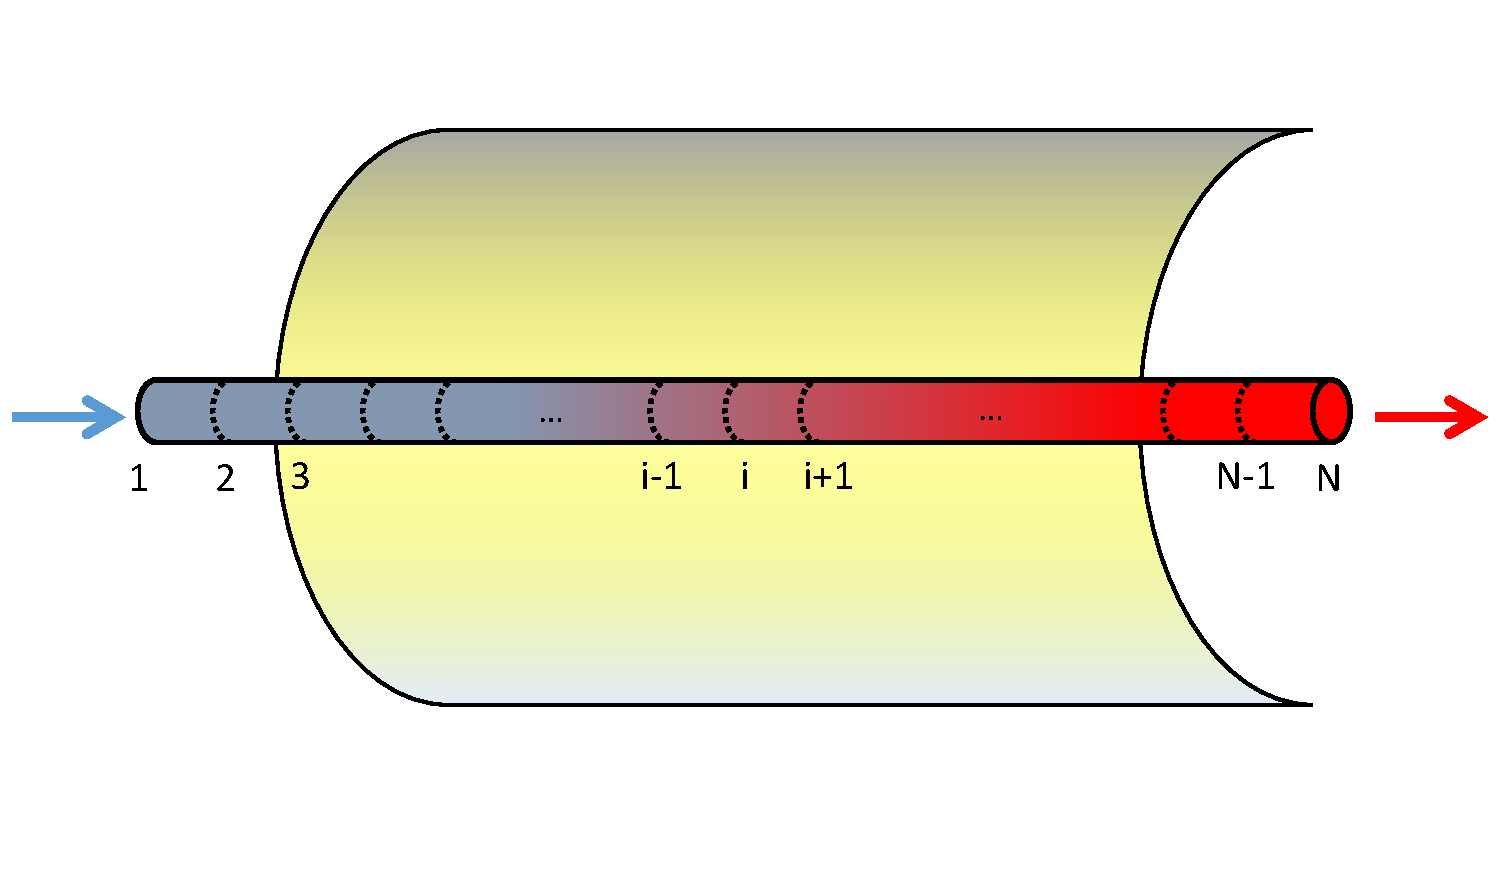
\includegraphics[width=0.95\textwidth]{Figures/PTC_FV.pdf}
		\caption{}
		\label{fig:PTC_FV}	
	\end{subfigure}
	\begin{subfigure}[b]{0.48\textwidth}
		\centering
		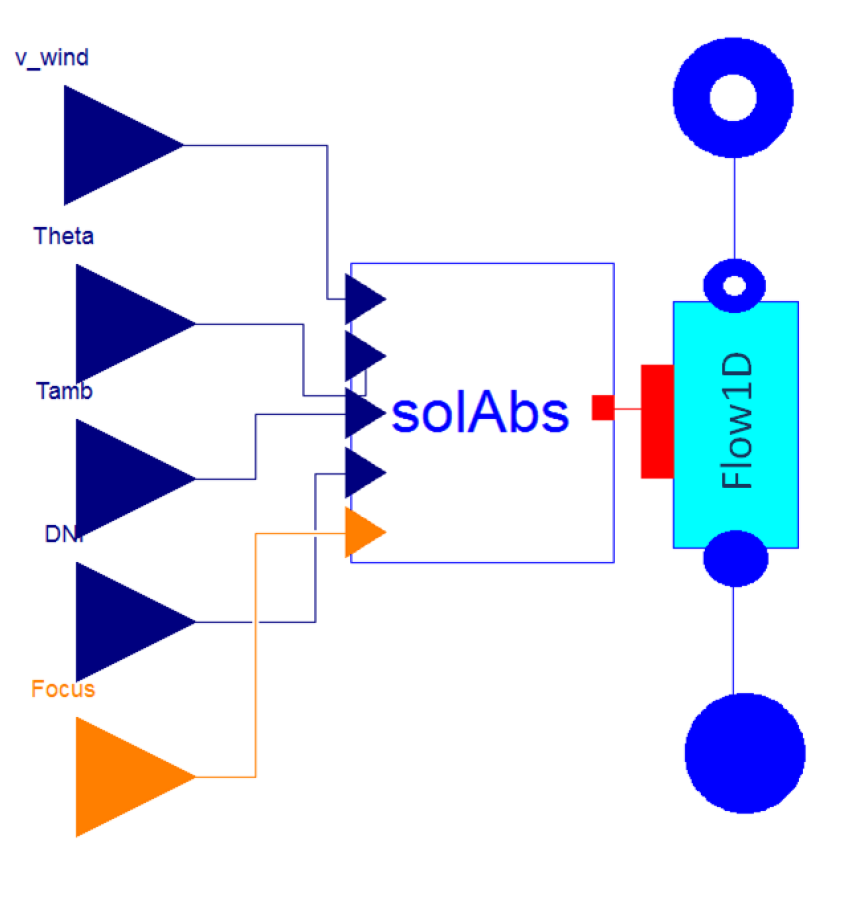
\includegraphics[width=0.7\textwidth]{Figures/PTC_GUI}
		\caption{}
		\label{fig:PTC_GUI}
	\end{subfigure}
	\caption{Parabolic trough collector model in ThermoCycle. \ref{fig:PTC_FV}: One-dimensional finite-volume modelling of the PTC. \ref{fig:PTC_GUI}: Object diagram of the solar collector model from the GUI of Dymola.}
	\label{fig:PTC_model}
\end{figure}
%
Following the object-oriented formalism of Modelica, the PTC model is built by interconnecting two sub-components, i.e. the \textit{Flow1D} and the \textit{SolAbs} models. These two sub-models are linked together through a thermal port as depicted in Figure~\ref{fig:PTC_GUI}.\\

The \textit{Flow1D} component simulates the HTF flow in the absorber tube. In each cell, both mass and energy balances are solved assuming an incompressible fluid and a static momentum balance , i.e.

\begin{align}
\frac{dM}{dt} & = \dot{m}_{su}-\dot{m}_{ex} = 0 \\
\frac{dM}{dt} & = V \left( \frac{\partial \rho}{\partial h}  \cdot \frac{dh}{dt} + \frac{\partial \rho}{\partial p} \cdot \frac{dp}{dt} \right) \\
V\rho \frac{dh}{dt} & = \dot{m}_{su}(h_{su} - h) - \dot{m}_{ex}(h_{ex} - h) + V \frac{dp}{dt} + A \cdot \dot{q}_{conv,fl} \\
p_{su} & = p_{ex}
\end{align}
where $\partial \rho / \partial h$ and $\partial \rho / \partial p$ are thermodynamic properties of the fluid directly computed by the open-source CoolProp library [ref]. The ''su'' (supply) and ''ex'' (exhaust) subscripts denote the nodes variable of each cell, $A$ is the lateral surface through which the heat flux $\dot{q}_{conv,fl}$ is transferred to the fluid and $V$ is the constant volume of each cell. Specific enthalpy and pressure at the center of the control volume are considered as the state variables. The different cells are interconnected to each other following an upwind discretization scheme. In each cell, the effective heat transfer to the fluid is given by the \textit{SolAbs} submodel. It is based on Forristall's steady-state model ~\cite{Foristall2003} and implements the dynamic radial energy balance between the heat collection elements and the ambiance, see Figure~\ref{fig:Forristal_cs2}. The model rely on physics-based equations and accounts for every physical phenomena in the heat balance, i.e.
\begin{itemize}
\item convection in the heat transfer fluid;
\item both conduction and thermal energy accumulation in the metal pipe;
\item both convection and radiation between the glass envelope and the metal pipe;
\item conduction and thermal energy accumulation in the glass envelope;
\item radiation and convection losses to the environment.
\end{itemize}
%
\begin{figure}[h!]
\centering
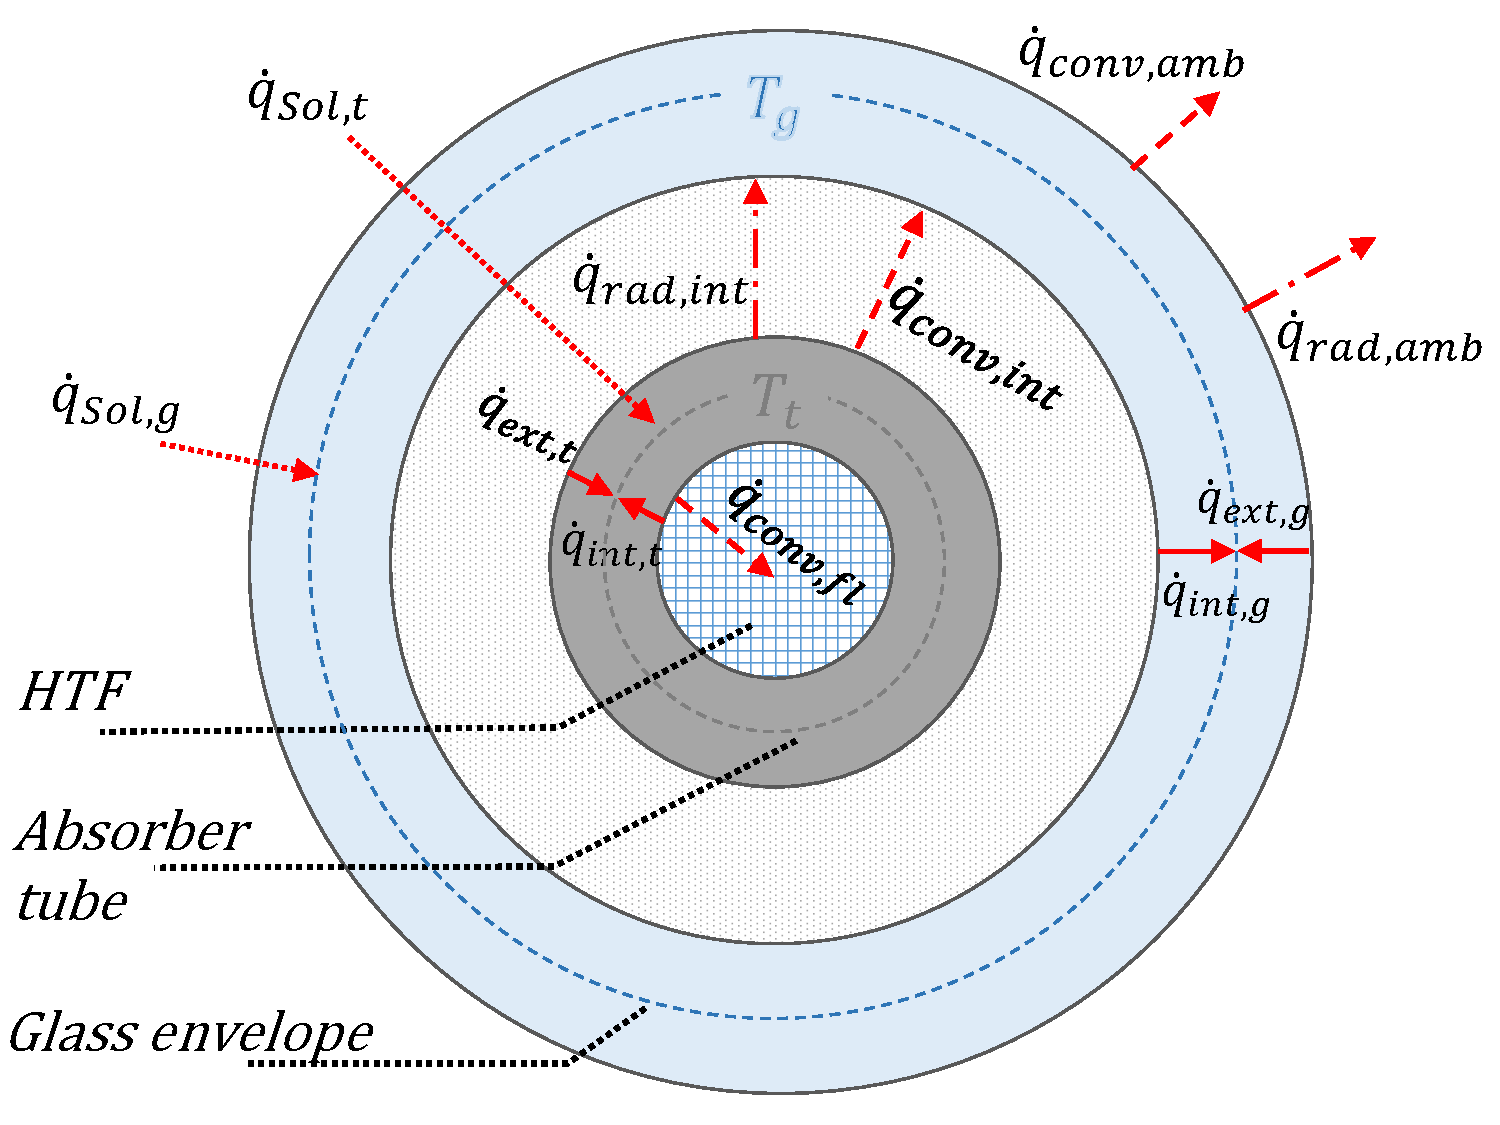
\includegraphics[width=0.5\textwidth]{Figures/Forristal_cs2.pdf}
\caption{Dynamic energy balance between the heat collection elements}
\label{fig:Forristal_cs2}
\end{figure}
%
Such approach permits to simulate the relationship between the environmental parameters (DNI , $\Theta_{incid}$, $T_{amb}$, $v_{wind}$) and the axial temperature distribution along the absorber tube. The thermal power transferred to the fluid ($\dot{q}_{conv,fl}$), the losses to the environment ($\dot{q}_{conv,amb} + \dot{q}_{rad,amb}$) and the temperatures of both the metal pipe ($T_{t}$) and the glass envelope ($T_{g}$) can then be evaluated. Regarding the main simulation assumptions, all the temperatures, heat transfers and thermodynamic properties are considered uniform around the circumference of the HCE (1D model). Heat losses through the support brackets are neglected and  solar absorptions in the tube and the glass envelope are treated as a linear phenomenon. Unlike Forristall's original model, the energy balance in the glass envelope and the metal pipe is calculated while accounting for their thermal capacitance, i.e.
\begin{align}
\rho_g C_{p,g} \frac{d T_g}{dt} & = \dot{q}_{int,g} D_{int,g} \pi + \dot{q}_{ext,g} D_{ext,g} \pi \\
\rho_t C_{p,t} \frac{d T_t}{dt} & = \dot{q}_{int,t} D_{int,t} \pi + \dot{q}_{ext,t} D_{ext,t} \pi
\end{align}
For a detailed description of all the heat transfer equations between the different elements, please refer to~\cite{Foristall2003} orÓ~\cite{Desideri2016thesis}. 


\section{Measurements and experiments}
\subsection{Experimental facility}
%
An aerial view of the PTTL system is shown in Figure \ref{fig:PTTL_photo}.
%
\begin{figure}[h!]
\centering
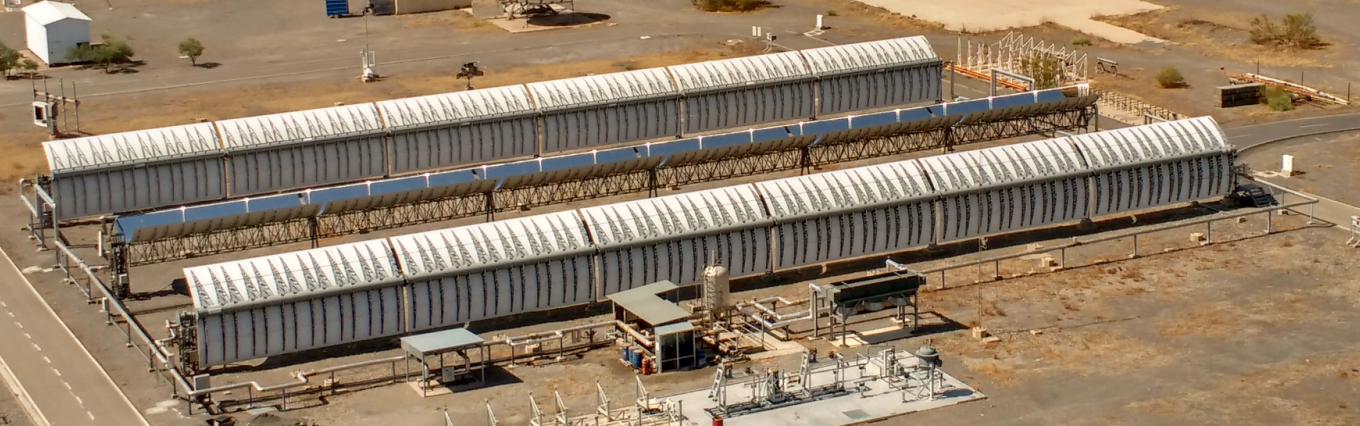
\includegraphics[width=1\textwidth]{Figures/SolarFieldTestRig_II.PNG}
\caption{Aerial view of the PTTL facility at PSA, Almer\' ia}
\label{fig:PTTL_photo}
\end{figure}
%
The solar field was characterized by three parallel lines of parabolic trough collectors (PTC) from different manufacturers AlbiasaTrough, EuroTrough and UrssaTrough. The system was a closed loop, with an East-West orientation and it is charged with the thermal oil Syltherm 800 \cite{DowOilandGas1997}. The process flow diagram of the PTTL facility is shown in Figure \ref{fig:PTTL_PI}. Looking at the bottom of Figure \ref{fig:PTTL_PI} it is possible to recognize the pump which drove the fluid, in liquid state, through one of the three parallel PTC lines of the solar field. The fluid was heated from (2) to (3) by absorbing the solar energy reflected by the collectors to the receiver tubes. At the outlet of the collectors the fluid was cooled down by air-cooler II characterized by a maximum thermal capacity of 400 kW$_{th}$. Once cooled down the oil reached the pump suction port (1). A 1 m$^3$ expansion vessel with Nitrogen, N$_\mathrm{2}$, inertization placed in between the two air coolers was used to regulate the loop pressure which was limited to 18 bar. In the whole circuit the oil was maintained in liquid state. Two electric heaters installed at the outlet of the pump allowed controlling the temperature of the oil at the inlet of the PTC lines. A mass flow meter at the outlet of the pump was used to measure the oil mass flow rate. The temperatures at the inlet and at the outlet of the PTC were measured with temperature transmittance (TT) sensors. The direct normal irradiance (DNI) was measured with a pyrheliometer model CH1 by Kipp\& Zonen \cite{Kipp1997}. A weather station installed nearby the solar field was used to measure the ambient temperature and the wind speed. The sensors signal outputs were acquired by a data acquisition system with a sampling time of 5 seconds and LabView was used for data visualization. 
%
\begin{figure}[h!]
\centering
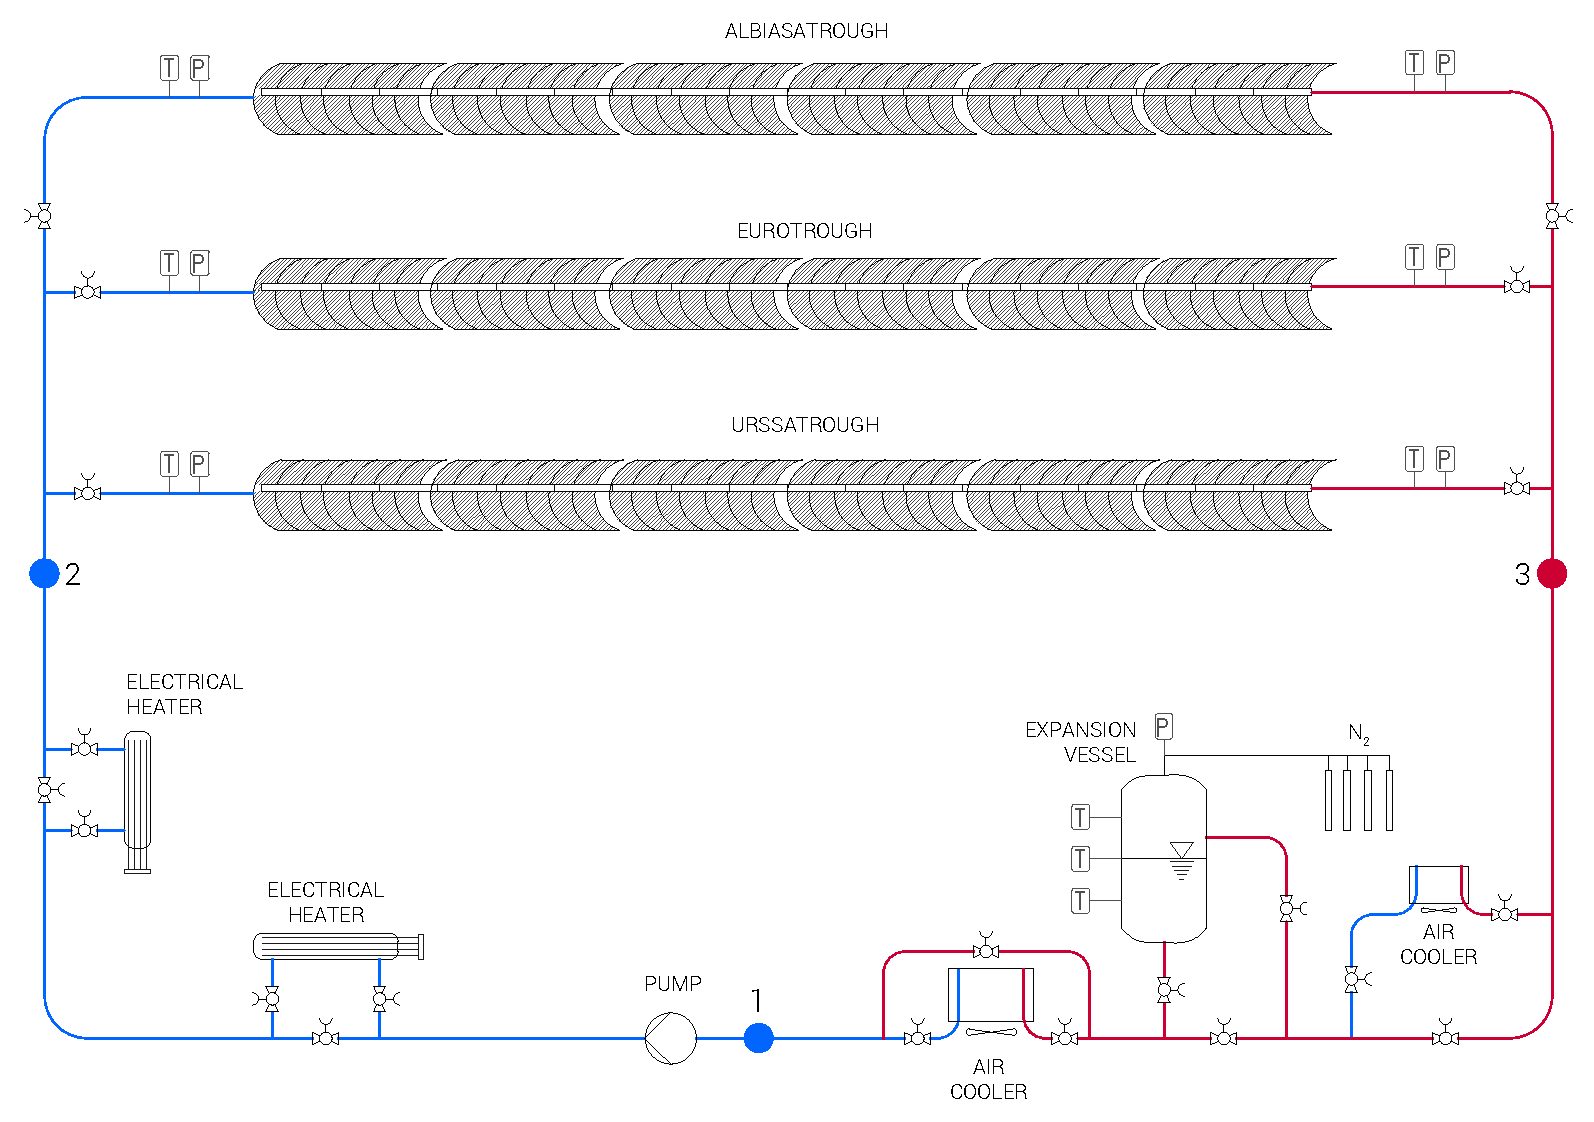
\includegraphics[width=1\textwidth]{Figures/SchematicSF_V2.pdf}
\caption{Process flow diagram of the PTTL facility with the relative sensors positions.}
\label{fig:PTTL_PI}
\end{figure}
%
During the experimental campaign on the PTTL facility, the EuroTrough collectors (ETC) line was tested. The ETC line was composed by 6 EuroTrough modules connected in series and 18 prototype receiver tubes from a Chinese manufacturer for a total length of 70.8 m and a net aperture area of 409.9 m$^2$.
%
\subsection{Dynamic experiments}
%
In order to characterize the dynamic performance of the ETC, the facility was run at different operating conditions by varying the pump speed velocity and the temperature at the inlet of the ETC for a total of 5 days of testing. In Table \ref{Tab:SF_workCond}, the working conditions ranges of the main variables and of the external ambient conditions during the experimental campaign are reported. 
%
\begin{table}[h!]
\centering
\caption{Range of operation of the ETC main variable and of the external ambient condition during the experimental campaign.}
\begin{tabular}{lccccccc}
\toprule
 Variable & $\dot{m}_\mathrm{oil,su}$ & p$_{SF,su}$  &T$_\mathrm{oil,su}$  & T$_\mathrm{oil,ex}$ &  DNI &  T$_\mathrm{amb}$ & v$_\mathrm{wind}$ \\
Unit &  [ kg s$^{-1}$] & [bar] & [$^{\circ}$C] &  [$^{\circ}$C]&  [$W$ m$^{-2}$] &  [$^{\circ}$C] &  [m s$^{-1}$] \\
\toprule
Min & 1.55      &   12.96 & 150.05  &   170.21  &   593.95  &   26.23 &   0  \\
Max & 5.03      &   16.07 & 304.48  &   352.28  &   883.72  &   33.16 &   11.23  \\
\bottomrule
\end{tabular}
\label{Tab:SF_workCond}
\end{table}
%
The dynamic validation was based on three specific sets of experiments:
%
\begin{itemize}
\item \textbf{MFE} - Oil mass flow change experiment: a step change was imposed to the oil mass flow rate at the inlet of the ETC by varying the pump speed velocity upwards or downwards starting from a steady-state condition.
\item \textbf{TE} - Oil inlet temperature change experiment: the oil temperature at the inlet of the ETC was varied by shutting down the air cooler starting from a steady-state condition. 
\item \textbf{SBE} - Solar beam radiation change experiment: a step change to the solar beam radiations  collected on the receiver was imposed downwards and upwards to the parabolic trough collectors by defocusing and focusing the parabolic trough collectors.
\end{itemize} 
%
\section{Simulation results and experimental validation}
%
The steady-state and dynamic validation of the parabolic trough solar field (SF) dynamic model described in section \ref{Sec:DynModel} is presented in this section. The model is compared against experimental data acquired on the PTTL facility at the Plataforma Solar de Almer\' ia (PSA), Spain. 
%
\subsection{Initial conditions, model inputs and parameters}
%
\label{subsec:SF_model}
In order to compare the acquired dynamic experimental data with the modelling results a simulation framework was defined. A schematic representation of the system is shown in Figure \ref{fig:SF_ModModel}. It comprised a mass flow source and a pressure sink connected to the fluid connectors of the SF model. 
%
\begin{figure}[h!]
\centering
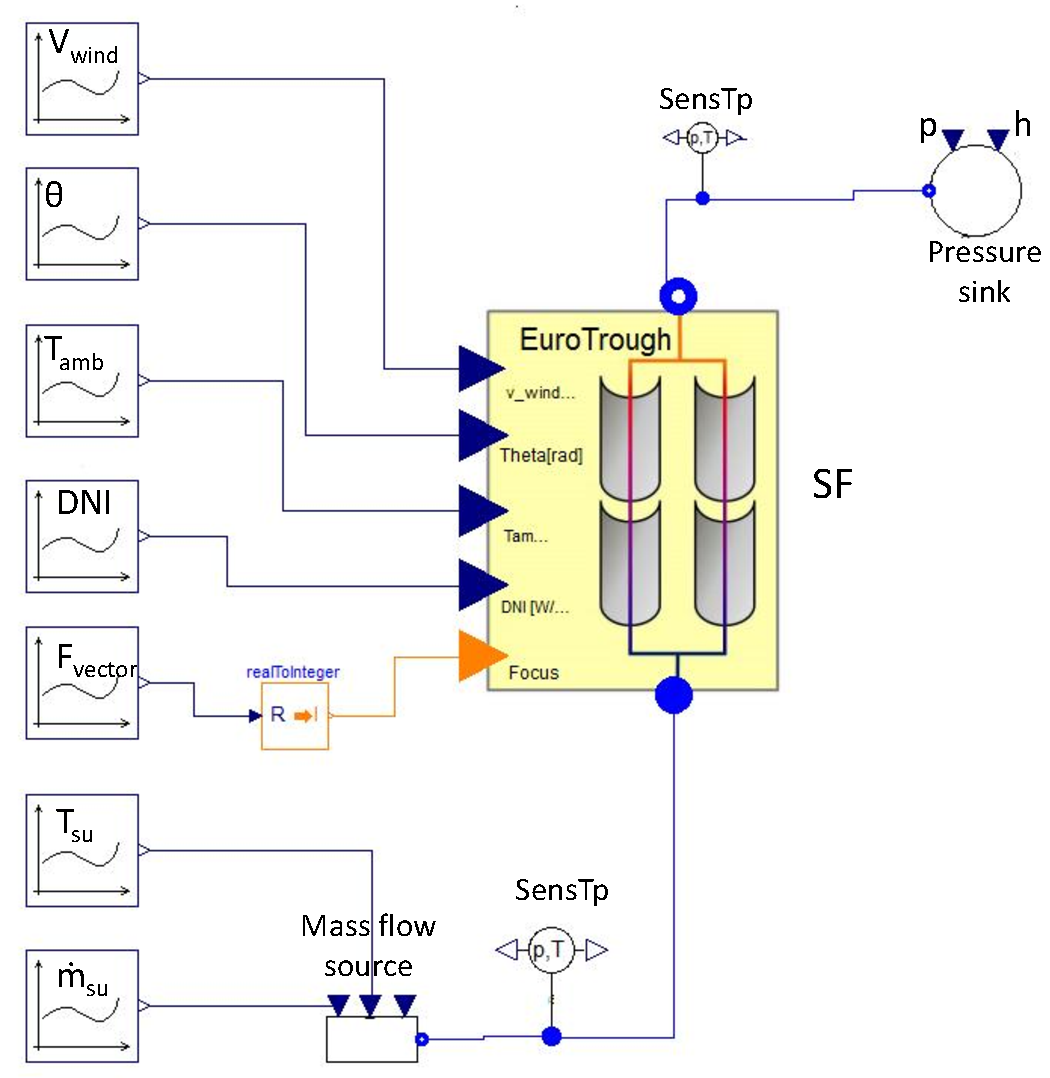
\includegraphics[width=0.6\textwidth]{Figures/Modelica_SF_v1crop.pdf}
\caption{Modelica model of the Eurotrough collector line installed in the PTTL facility from the Dymola graphical user interface (GUI).}
\label{fig:SF_ModModel}
\end{figure}
%
The exogenous inputs (EI) imposed to the SF model and the relative unit are listed in Table \ref{Tab:SF_Inputs}. 
%
\begin{table}[h!]
\centering
\caption{List of exogenous inputs (EI) imposed to the SF model.$v_{wind}$: wind speed, $\Theta_\mathrm{incid}$: solar radiation incidence angle, $T_{amb}$: ambient temperature, DNI: direct normal irradiance, $F_{vector}$: vector for defocusing action, $\dot{m}_{oil,su}$: oil mass flow at SF inlet,  $T_{oil,su}$: oil temperature at SF inlet, $p_{ex}$: oil pressure at SF outlet}
\begin{tabular}{lcccccccc}
\toprule
EI   & v$_\mathrm{wind}$   & $\Theta_\mathrm{incid}$ & $T_\mathrm{amb}$      & DNI                & $F_\mathrm{vector}$   & $\dot{m}_\mathrm{oil,su}$ & $T_\mathrm{oil,su}$   & $p_\mathrm{ex}$ \\
Unit & [m s$^{-1}$] & [Rad]    &  [$^{\circ}$C] &  [$W$ m$^{-2}$]      & [-]            &  [kg s$^{-1}$]     &  [$^{\circ}$C] &  [bar] \\
\bottomrule
\end{tabular}
\label{Tab:SF_Inputs}
\end{table}
%
The SF model was parametrized based on the data-sheets of the EuroTrough collector and the receiver tubes. The incidence angle modifier (IAM), required for the optical efficiency calculation, was computed with an empirical equation as:
%
\begin{equation}
IAM = 1 - \frac{a_\mathrm{I} \cdot \Theta_\mathrm{incid} + a_\mathrm{II}\cdot \Theta_\mathrm{incid}^2}{\cos{\Theta_\mathrm{incid}}}
\end{equation} 
%
where $\Theta_\mathrm{incid}$ is the incidence angle of solar radiation and $a_\mathrm{I}-a_\mathrm{II}$ are two empirical parameters derived through an experimental campaign as described in \cite{Sallaberry2016} following the methodology presented in \cite{Valenzuela2014}. In order to consider unaccounted optical effects during testing, e.g., dirt on the parabolic mirrors and tube receivers, the parameter $\epsilon_\mathrm{un}$ was included in the calculation of the optical efficiency. Its value was obtained through a least square optimization routine aimed at minimizing the error between the simulated SF outlet temperature and the measured one over a three minutes interval  of the initial steady-state condition characterizing the first day of testing (see Figure \ref{fig:SF_ModRes_All}). In Table \ref{tab:SF_parameter} the values assigned to the parameters of the SF model are reported.
%
\begin{table}[h]
  \centering
  \caption{Values of the parameters for the SF Modelica model}
    \begin{tabularx}{\textwidth}{Xcc}
    \toprule
    Parameter & Units & Value \\
\midrule 
   General parameters &  &  \\
   \hspace*{0.3cm} N - Number of discretized cells  & [-]    & 20 \\
   \hspace*{0.3cm} L - PTC length   & [m]    & 70.8 \\
   \hspace*{0.3cm} A$_\mathrm{p}$ - Parabola aperture & [m]    & 5.76 \\
   Optical properties &  &  \\   
   \hspace*{0.3cm} $\rho_{cl}$ - Mirror reflectivity & [-]    & 0.9388 \\
   \hspace*{0.3cm} $\tau_{gl}$ - Glass transmissivity & [-]    & 0.92 \\
   \hspace*{0.3cm} $\alpha_{gl}$ - Glass absorptivity  & [-]    & 0.02 \\
   \hspace*{0.3cm} $\epsilon_{gl}$ - Glass emissivity & [-]   & 0.86 \\
   \hspace*{0.3cm} $\alpha_{tu}$ - Tube Absorptivity & [-] & 0.7919 \\
   \hspace*{0.3cm} $a_\mathrm{I}$ - IAM coefficient I & [-] & 4.11$e^{-3}$ \\
   \hspace*{0.3cm} $a_\mathrm{II}$ - IAM coefficient II & [-] & 5.513$e^{-5}$ \\
   \hspace*{0.3cm} $\epsilon_\mathrm{un}$ - Unaccounted & [-] & 0.9437 \\
   Glass envelope geometries &  &  \\
   \hspace*{0.3cm} D$_{gl}$ - External glass diameter & [m] & 0.12\\
   \hspace*{0.3cm} t$_{gl}$ - Glass thickness  & [m] & 0.0025\\
   Receiver tube geometries &  &  \\
   \hspace*{0.3cm} D$_{tu}$ - External glass diameter & [m] & 0.07\\
   \hspace*{0.3cm} t$_{tu}$ - Glass thickness  & [m] & 0.002\\
    Vacuum properties &  &  \\
   \hspace*{0.3cm} p$_{vacuum}$ - Vacuum pressure & [bar] & 1.333$e^{-7}$\\
   \hspace*{0.3cm} $\Gamma$ - Ratio of specific heats for the annulus gas & [-] & 1.39\\
   \hspace*{0.3cm} $\Delta_{mol}$ - Molecular diameter for the annulus gas & [m] & 3.53$e^{-10}$\\
   \hspace*{0.3cm} $k_\mathrm{std}$ - Thermal conductivity at standard pressure and temperature & [W m$^{-1}$K$^{-1}$] & 0.02551\\
    \bottomrule
    \end{tabularx}%
  \label{tab:SF_parameter}%
\end{table}%
%
The \textit{GlassUD} and \textit{TubeUD} options were set to false such that the density, specific heat capacity and thermal conductivity of the glass and the metal tube were computed as dependent on the glass and tube temperatures respectively.
The heat transfer coefficient was computed based on the Gnielinski single phase correlation \cite{Gnielinski2010}.
The thermal oil, Syltherm 800, flowing through the tube receivers was modelled as an incompressible fluid using the \textit{TableBased} framework of the Modelica Standard library. As a consequence no mass accumulation was considered in the receiver tubes.
% How we modelled the heat transfer coefficient....


%
\subsection{Results:Steady-state validation}
%


%
The SF Modelica model was run on Dymola2015. The Differential Algebraic System Solver (DASSL) \cite{Petzold1983} was selected as numerical solver, setting the relative tolerance to 10$^{-4}$. In order to increase the model robustness and decrease the computational time, the measured variables imposed as exogenous inputs to the SF model (see Table \ref{Tab:SF_Inputs}) are approximated by a spline function in the Modelica/Dymola simulation environment.\\
In Figure \ref{fig:SF_ModRes_Zoomed}, the simulated ETC outlet temperature is plotted versus time and compared against the measured data for each of the three performed dynamic experiments. On the left abscissa the measured ETC inlet and outlet temperatures and the simulated ETC outlet temperature are plotted versus time. On the right abscissa the DNI and oil mass flow rate normalized with respect to the maximum value reached during the day are reported. For all the plots it is possible to see how the DNI was characterized by variation smaller than 2\%. In Figure \ref{fig:SF_ModRes_Zoomed}a the results for the MFE experiments and simulation results are reported. Starting from a steady-state condition two consecutive steps of the same magnitude upwards and downwards were imposed to the pump rotational speed at t=450 seconds and t=1430 seconds respectively. As the rotational speed increased at t=450 seconds, the velocity and pressure of the fluid in the high pressure line increased. This resulted in an oil mass flow rate, $\dot{m}_\mathrm{oil,su}$, increment of about 40\% in around 60 seconds. The increase in oil mass flow rate caused a drop in the temperature at the outlet of the ETC, $T_\mathrm{oil,ex}$. The $T_\mathrm{oil,ex}$ drop was registered at around t=500 seconds, 50 seconds after the oil mass flow rate started changing. This was due to the time required by the oil mass flow rate to reach the outlet of the 70.8 m long receiver tubes. During the experiments the ETC inlet temperature, $T_\mathrm{oil,su}$, was maintained constant  by manually manipulating the air cooler and electrical heaters power. 
When the oil mass flow rate was changed upwards, as $T_\mathrm{oil,su}$ was expected to decrease the air cooler power was 
decreased and the electrical heaters power was increased manually, causing a small bump within 2 K in the temperature as it is shown in Figure \ref{fig:SF_ModRes_Zoomed}a.  
The same phenomena in the opposite direction took place when the pump speed was decreased. 
The ETC outlet temperature presented a symmetrical trend for the upwards and downwards oil mass flow rate change. The SF model was able to well predict the experimental trend both for the upward and downward steps and was characterized by a time constant slightly smaller than the real system.\\
In Figure \ref{fig:SF_ModRes_Zoomed}b the TE experiments and simulation results are reported. Starting from a steady-state condition the air-cooler was turned off at t=900 seconds. This resulted in an increase of $T_\mathrm{oil,su}$ and a consequently growth of $T_\mathrm{oil,ex}$ delayed by around 100 seconds due to the time required by the oil mass flow to travel through the tube receiver. The shut-down of the oil-cooler did not allow to impose a step to $T_\mathrm{oil,su}$ which increased with a slow first order trend. The large time constant characterizing $T_\mathrm{oil,su}$ defined the change of the outlet ETC temperature. The SF model was able to correctly predict the experimental results including  the delay characterizing the $T_\mathrm{oil,ex}$ change.\\
Finally in Figure \ref{fig:SF_ModRes_Zoomed}c the SBE experiments and simulation results are shown. Starting from a steady-state condition the ETCs were defocused at t=360 seconds, such that no solar radiation was reflected to the receiver tubes. This caused a sudden decrease of $T_\mathrm{oil,ex}$ which reached the $T_\mathrm{oil,su}$ value in about 200 seconds. The ETCs were focused again at t=650 bringing $T_\mathrm{oil,ex}$ back to its initial value. During the experiment the oil mass flow rate and $T_\mathrm{oil,su}$ were kept constant. The latter was maintained at its initial value by manually manipulating the power of the two electrical heaters installed after the pump. This resulted in a small bump of less then 4 K after the collectors were focused at t=700 seconds. The $T_\mathrm{oil,ex}$ was characterized by a symmetrical behaviour during the focusing-defocusing experiments, as the thermal energy losses were relatively small. The SF model was able to replicate the trend and presented a slightly smaller time constant than the real system.\\
Overall it can be concluded that the SF Modelica model was capable of predicting the physical phenomena characterizing the real system behaviour during the three performed experiments and can be considered validated.
%
\begin{figure}[h!]
\centering
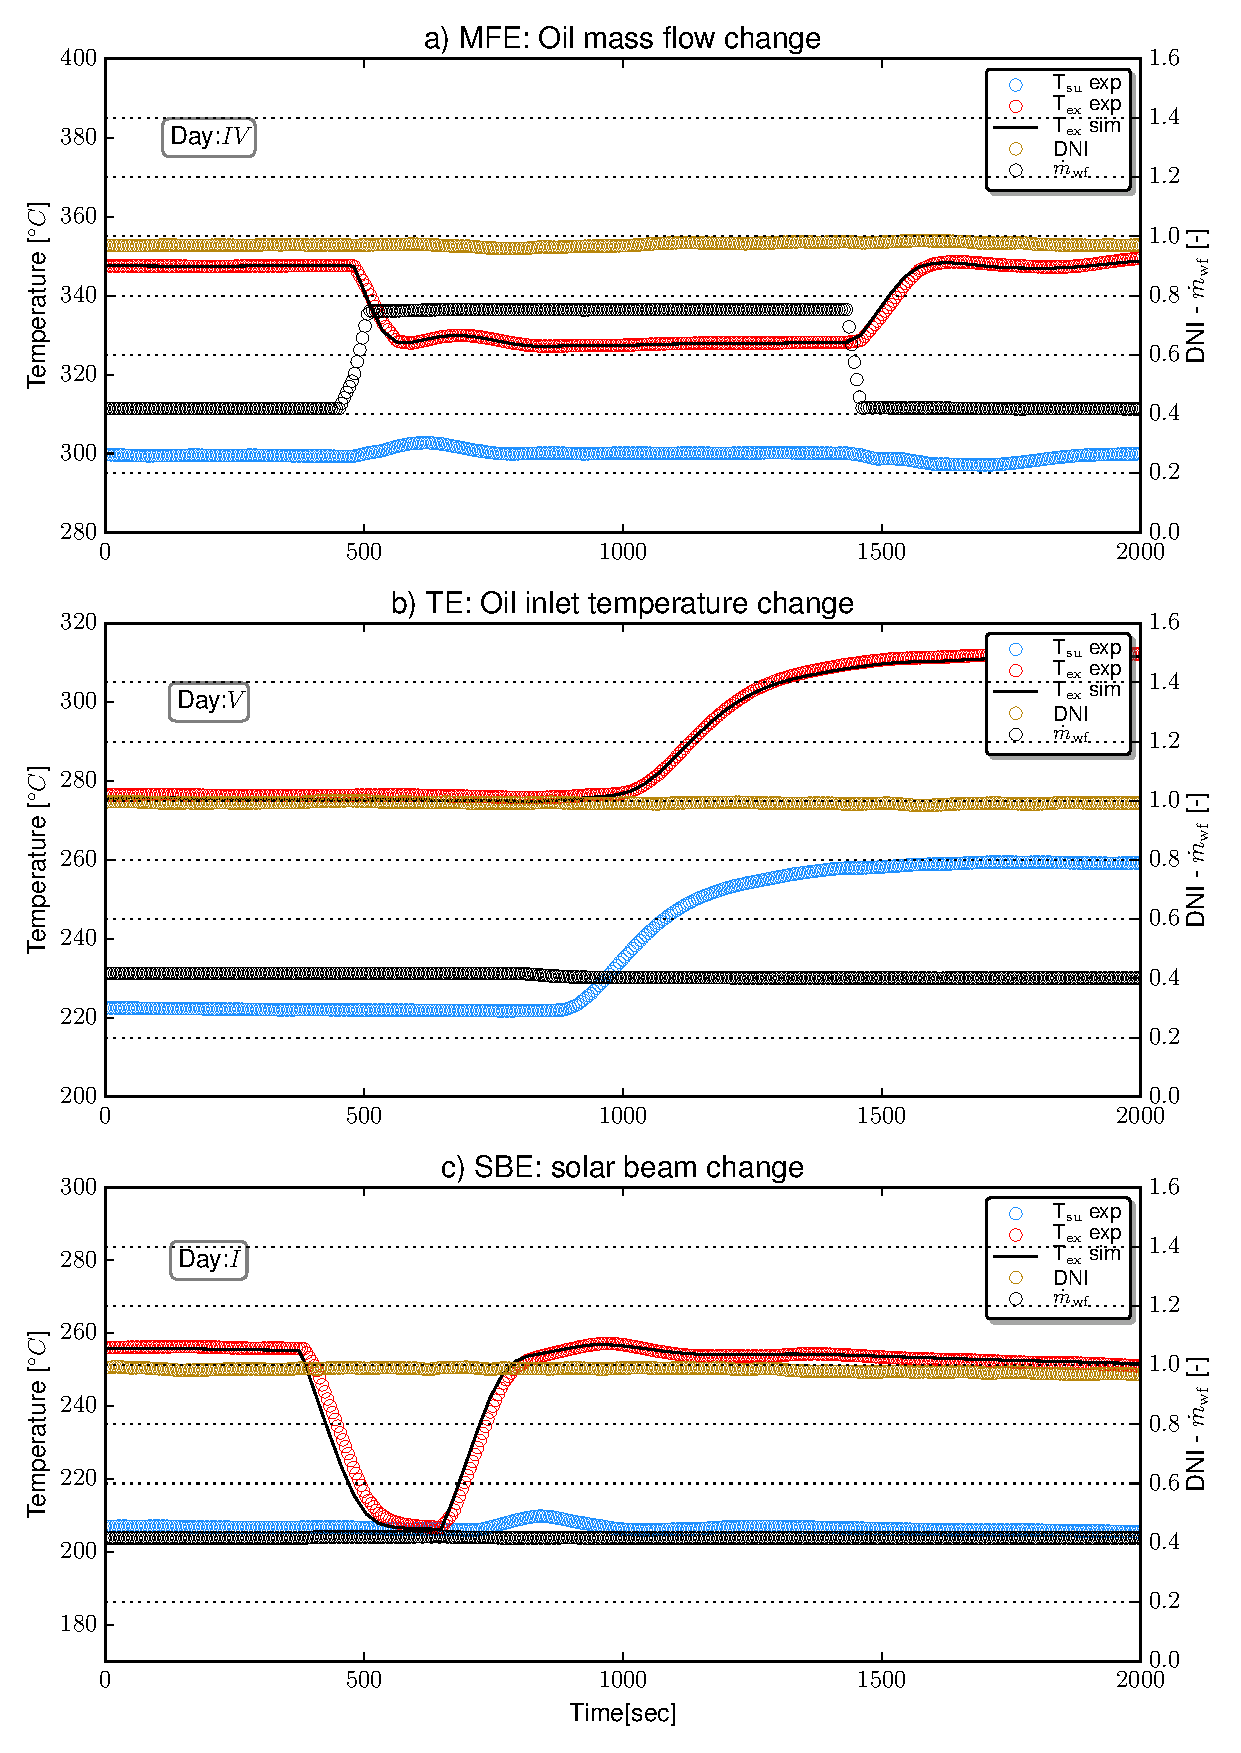
\includegraphics[width=0.95\textwidth]{Figures/_MassFlowChange.pdf}
\caption{Simulation and experimental results plotted versus time for: a) MFE - Mass flow change experiment  b) TE - inlet ETC temperature change experiment c) SBE - solar beam radiation change experiment. The measured inlet and outlet ETC temperatures and the outlet SF model temperature are plotted on the left abscissa. The normalized DNI and oil mass flow rate values are plotted on the right abscissa.}
\label{fig:SF_ModRes_Zoomed}
\end{figure}
%
In Figure \ref{fig:SF_ModRes_All} the simulation and experimental results for all of the five days of the experimental campaign are reported. In the first Figure, \textit{Day I}, the three minutes time over which the $\epsilon_\mathrm{un}$ parameter was optimized are highlighted by two vertical black dotted lines.
%
\begin{figure}[h!]
\centering
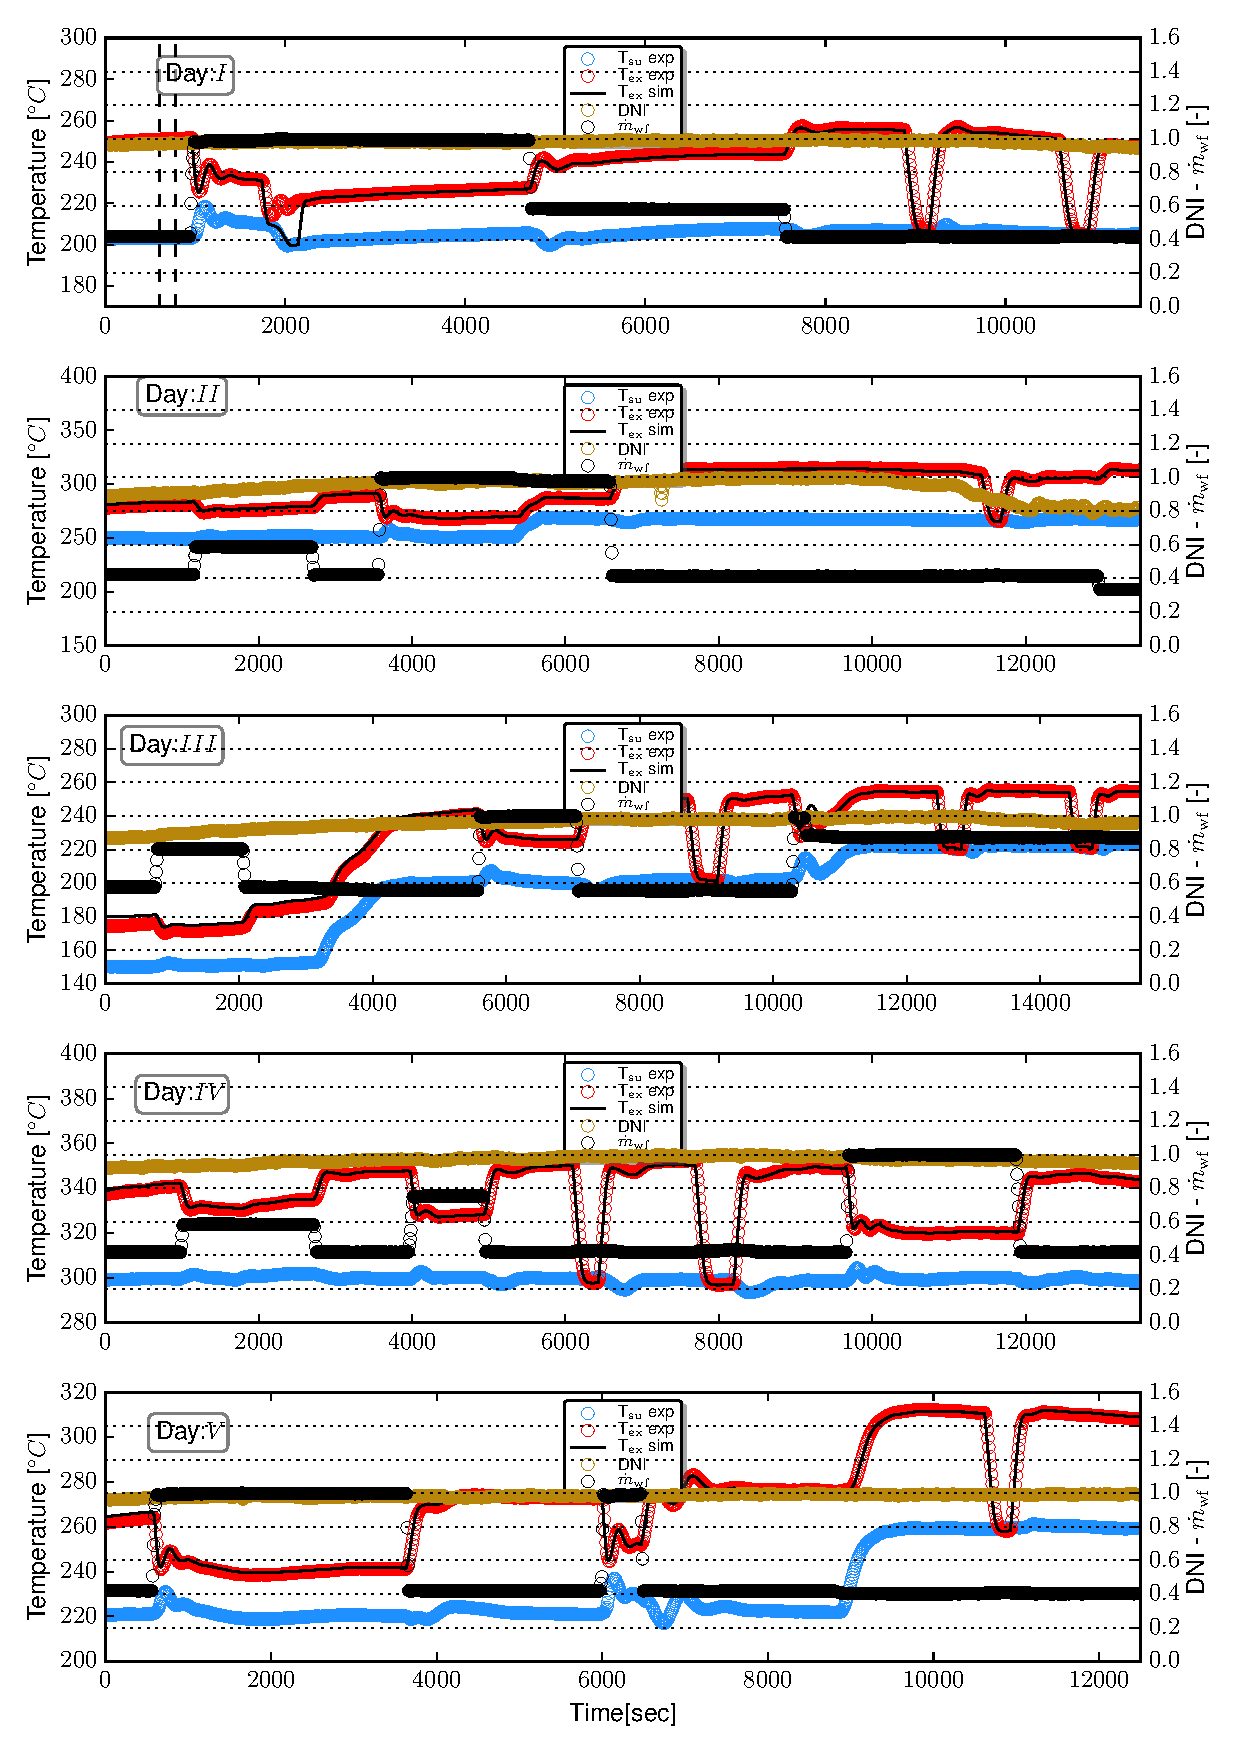
\includegraphics[width=1\textwidth]{Figures/_FirstFiveDays.pdf}
\caption{Simulation versus experimental results for each full day of the experimental campaign plotted versus time. }
\label{fig:SF_ModRes_All}
\end{figure}
%
\subsection{Results: number of tube receiver CVs parametric analysis } 
%
In order to investigate the effect of the level of discretization on the performance of the SF model when compared to the experimental results a parametric analysis was performed. The SF model, discretized with a number of control volumes (CVs) varying from 1 to 50,  was simulated to replicate the  experimental data of Day $IV$ (see Figure \ref{fig:SF_ModRes_All}). The results are displayed in Figure \ref{fig:SF_ModRes_ParAnalysis}a where the simulated SF outlet temperature for the different levels of discretization is plotted versus time and compared against the measured experimental data on the left abscissa. On the right abscissa the nominal DNI and oil mass flow rate are plotted. Overall as the level of discretization increased the SF outlet temperature got closer to the measurements data. From 10 to 50 CVs the improvement in model accuracy was negligible. On the other hand the 5 CVs and 1 CVs SF model presented a slower time constant compared to the real system and were not able to properly predict the different undershoot and overshoot characterizing the measured outlet ETC temperature when the boundary conditions where changed, e.g., step change in the mass flow or defocusing-focusing.\\
In Figure \ref{fig:SF_ModRes_ParAnalysis}b the percentage computational effort (PCE) defined in equation \ref{eq:PCE} as the ratio of the computational time (Time$_\mathrm{Comp}$) with respect to the simulated real time ($\mathrm{Time}_\mathrm{Real}$), is plotted for each simulation result. All the simulation results were characterized by a much shorter time compared to the real simulated time. This is related to the remarkably simple simulation framework on which the modelling results were based on (see section \ref{subsec:SF_model}). 
%
\begin{equation}
\mathrm{PCE} = \frac{\mathrm{Time}_\mathrm{Comp}}{\mathrm{Time}_\mathrm{Real}} \cdot 100
\label{eq:PCE}
\end{equation}
%
The computational time increased exponentially with the increase of number of CVs with the 1 and 5 CVs SF models being one order of magnitude faster than the higher discretized model.\\
In order to assess the discrepancy between the different CVs discretization levels, the total energy absorbed by the thermal oil in the ETC collectors, $E_\mathrm{oil}$,  was computed as the integral of the thermal power over the simulated time, around 4 hours, and compared with respect to the 50 CVs model which was taken as a reference. The percentage relative error $\bar{\epsilon}$ for each SF model was computed as:
%
\begin{equation}
\bar{\varepsilon}(k) = 100 \cdot \frac{|E_\mathrm{oil,50CVs} -E_\mathrm{oil,k}|}{E_\mathrm{oil,50CVs}}  \quad k \in [1,5,10,20]. 
\end{equation}
%
The results are reported in Table \ref{tab:SF_Etot}.
%
\begin{table}[h!]
  \centering
  \caption{Total energy percentage relative error for the different levels of discretization of the SF model.}
    \begin{tabular}{lc}
    \toprule
    Model & \multicolumn{1}{c}{$\bar{\varepsilon}$ [\%]}  \\
    \midrule
    SF CVs 1      & 0.5         \\
    SF CVs 5      & 0.18         \\
    SF CVs 10     & 0.08          \\
    SF CVs 20     & 0.03          \\   
    \bottomrule
    \end{tabular}%
  \label{tab:SF_Etot}%
\end{table}%
%
As it possible to see, the overall percentage relative error on the total energy absorbed by the fluid over 4 hours of simulation with respect to the 50 CVs SF reference model was negligible for all the tested levels of discretization.\\

%1 - 5 - 10 - 20 
% 0.50323002464612376, 0.1887974297686737, 0.08694895129959232, 0.03231713606505187
\begin{landscape}
\begin{figure}[h!]
\centering
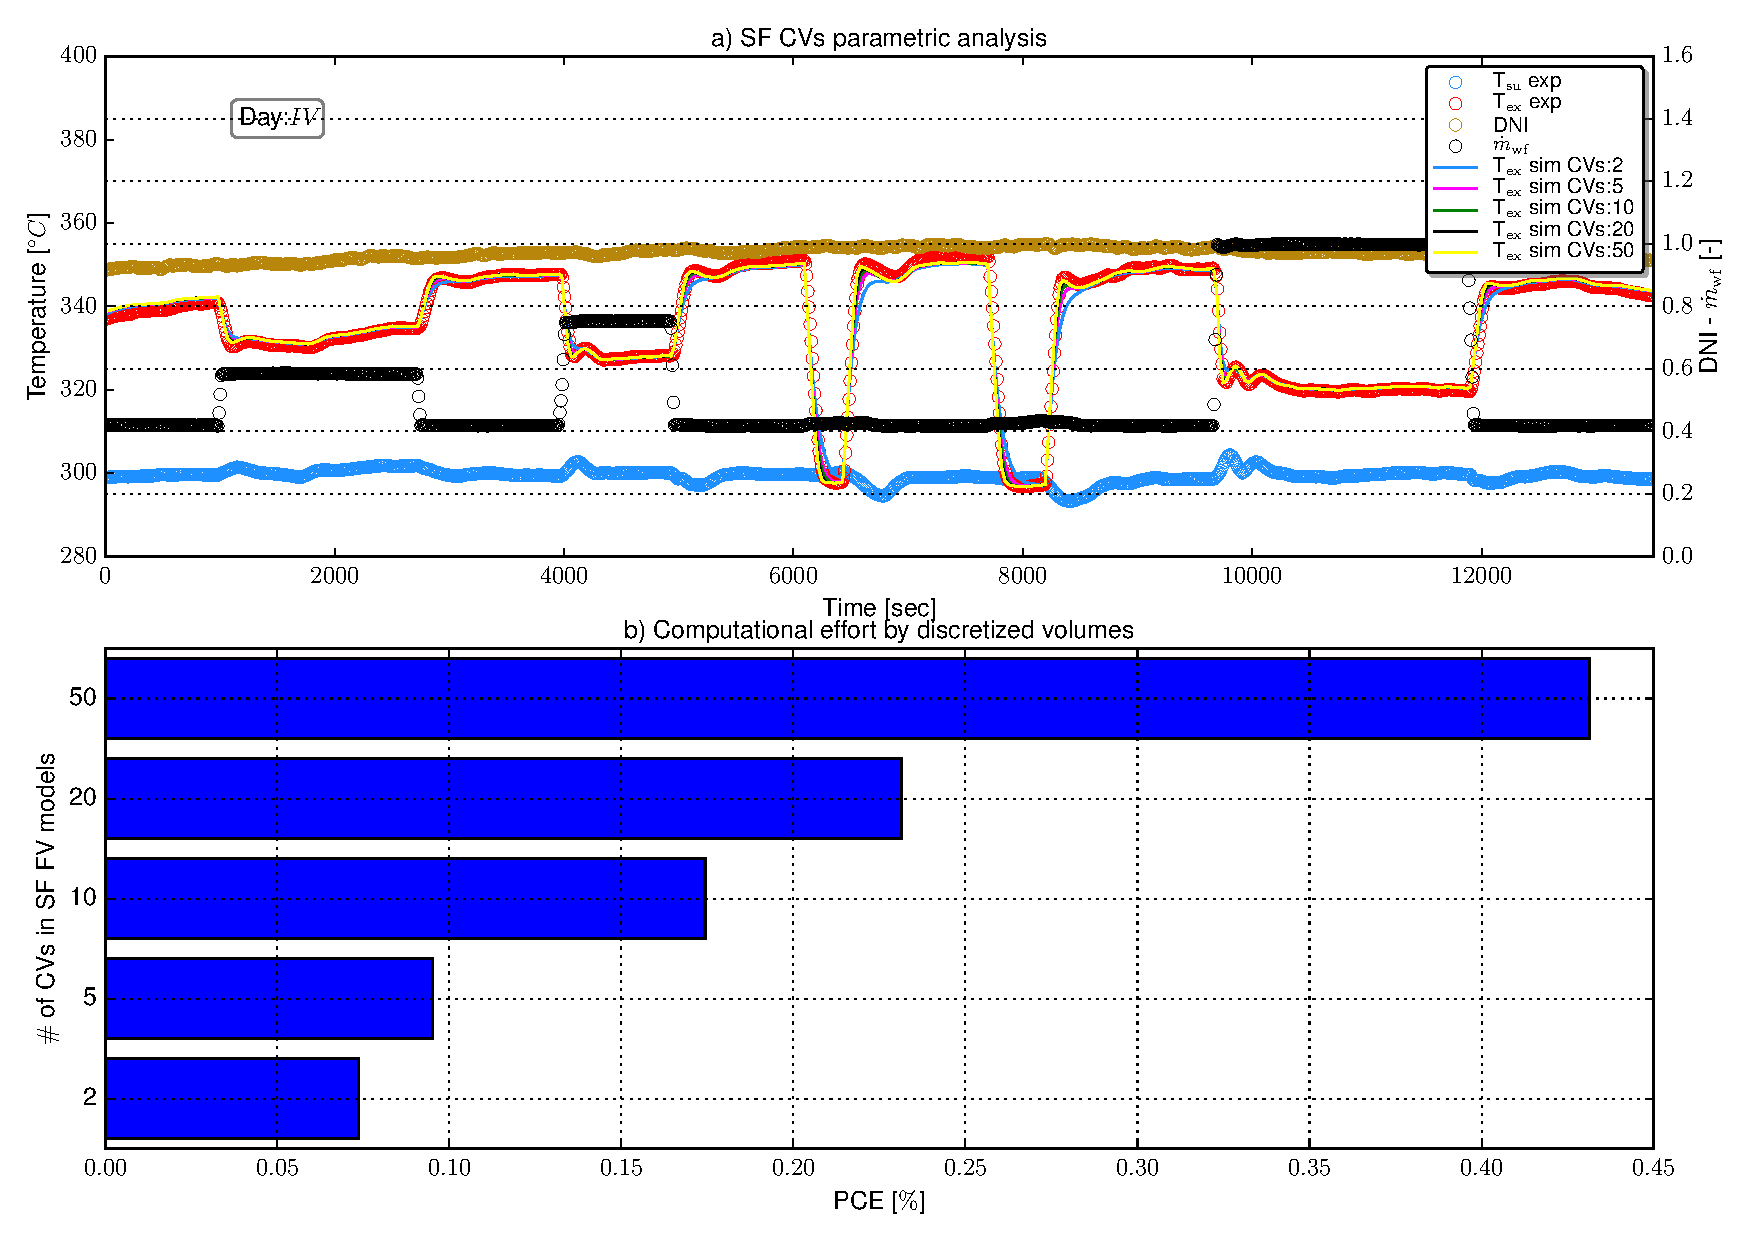
\includegraphics[height=0.95\textheight]{Figures/_SF_NodesParaALL.pdf}
\caption{Simulation results versus the experimental results for each full day of the experimental campaign. PCE: percentage computational effort.}
\label{fig:SF_ModRes_ParAnalysis}
\end{figure}
\end{landscape}
%
%
%
\section{Discussion}
%


%
\section{Conclusions}
%
The parabolic trough ThermoCycle Modelica model was compared against experimental data acquired on the PTTL facility at the Plataforma Solar de Almer\' ia (PSA), Spain. Dynamic experiments were performed by varying the oil mass flow rate (MFE), the oil inlet temperature (TE) and the direct beam solar radiation (SBE) for different operating conditions. 
%
\begin{itemize}
\item The simulation results obtained for the oil mass flow change experiment(MFE), the oil inlet temperature change experiment (TE) and the solar incidence beam radiation experiment (SBE) showed a good overlap with the experimental results. The developed solar field model structure proves to be effective to predict the dynamic of a real solar field.
%
%Based on these analyses the following conclusions can be drawn:
%\begin{itemize}
%\item The SF model structure proved effective to simulate parabolic trough collectors systems when subjected to change in the inlet mass flow rate (MFE), the inlet temperature (TE) and to variation of the solar beam (SBE).
%\item A minimum discretization level of 20 CVs is recommended if the ETC outlet temperature has to be precisely predicted, e.g., the  SF model is used as a reference to develop and test model based control strategies. 
%\item A single CVs is sufficient if the performance of the ETC collectors are analysed on a daily or longer basis. This approach allows to significantly decrease the computational time while maintaining a satisfying degree of accuracy.
%\end{itemize}
%
\item A minimum discretization level of 20 CVs was found to be a good compromise between model accuracy and simulation speed if the ETC outlet temperature had to be precisely predicted, e.g., the  SF model is used as a reference to develop and test model based control strategies.
%
\item In light of the obtained results a lumped SF model is recommended if the performance of the ETC collectors are analysed on a daily or longer time frame. This approach allows to significantly decrease the computational time while maintaining a satisfying level of accuracy.
\end{itemize}
%
It was proven that the modelling approaches adopted led to satisfactory results for the simulation of parabolic trough collector systems.\\
The proposed solar collector model together with the test cases is released as open-source and is available in the latest version of the ThermoCycle library.\\
%
%
%
\section{Acknowledgements}
%
The results presented in this paper have been obtained within the frame of the SFERA II project.
%
\clearpage
%\bibliographystyle{model3-num-names}
%\bibliography{Solar}


\end{document}
\endinput



